%%%%%%
%
% $Autor: Wings $
% $Datum: 2020-01-18 11:15:45Z $
% $Pfad: githubtemplate/Template/Presentations/Template/slides/rename.tex $
% $Version: 4620 $
%
%
% !TeX encoding = utf8
% !TeX root = Rename
%
%%%%%%



\section{TensorFlow Lite}

\STANDARD{TensorFlow Lite}
{ 
	
  \framesubtitle{Overview}
\begin{itemize}
	\item What is TensorFlow Lite?
	\begin{itemize}
		\item TensorFlow Lite is a lightweight version of TensorFlow, which is an open-source machine learning framework developed by Google. 
		\item TensorFlow Lite is specifically designed for mobile and edge devices, allowing machine learning models to run efficiently on smartphones, embedded systems, and other devices with limited computational resources.
		\item TensorFlow Lite optimizes machine learning models for deployment on these devices by providing tools for model conversion, model optimization, and inference.
	\end{itemize}
\end{itemize}
}

\section{Benefits of TensorFlow Lite}
\STANDARD{Benefits of TensorFlow Lite}
{ 
	\framesubtitle{Key benefits}	
		\begin{itemize}
			\item Low Latency: Faster inference on-device.
			\item Reduced Size: Smaller model and binary sizes suitable for devices with limited resources.
			\item For common machine learning tasks such as image classification, object detection, pose estimation, question answering, text classification, etc. on multiple platforms.
		\end{itemize}
}

\section{Core Components of TensorFlow Lite}
\STANDARD{Core Components of TensorFlow Lite}
{ 
\begin{itemize}
	\item Interpreter: Executes the model.
	\item Converter: Converts TensorFlow models into a compressed flat buffer format.
	\item Supported Ops: Set of operations optimized for mobile and embedded devices.
\end{itemize}
}

\section{TensorFlow Lite Working}
\STANDARD{TensorFlow Lite Working}
{
	\begin{center}
	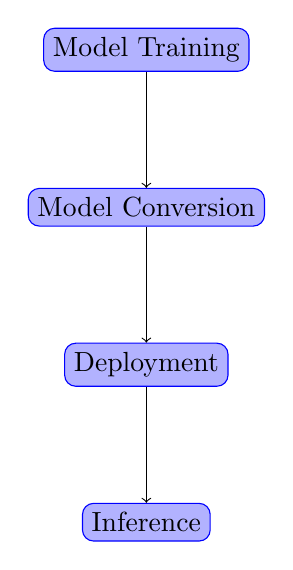
\begin{tikzpicture}[node distance=2cm, auto]
		% Nodes
		\node[rectangle, rounded corners, draw=blue, fill=blue!30] (training) {Model Training};
		\node[rectangle, rounded corners, draw=blue, fill=blue!30, below of=training] (conversion) {Model Conversion};
		\node[rectangle, rounded corners, draw=blue, fill=blue!30, below of=conversion] (deployment) {Deployment};
		\node[rectangle, rounded corners, draw=blue, fill=blue!30, below of=deployment] (inference) {Inference};
		
		% Arrows
		\draw[->] (training) -- (conversion);
		\draw[->] (conversion) -- (deployment);
		\draw[->] (deployment) -- (inference);
	\end{tikzpicture}
	\end{center}
}
\STANDARD{TensorFlow Lite Working}
{ 
	
	\framesubtitle{Step-by-Step working}	
	\begin{enumerate}
		\item Model Training:
		\begin{itemize}
			\item Train a model using TensorFlow on a desktop or cloud environment.
		\end{itemize}
		\item Model Conversion:
		\begin{itemize}
			\item Convert the trained model to TFLite format (.tflite) using the TFLite Converter
		\end{itemize}
		\item Deployment: 
		\begin{itemize}
			\item Deploy the TFLite model on mobile, embedded, or IoT devices.
		\end{itemize}
		\item Inference:
		\begin{itemize}
			\item Run the model using TFLite Interpreter to perform predictions on the device.
		\end{itemize}
	\end{enumerate}
}

\section{TF Lite Model Conversion}
\STANDARD{TensorFlow Lite Model Conversion}
{ 
	
	
\begin{itemize}
	\item \textbf{TFLite Converter}:
	\begin{itemize}
		\item The TensorFlow Lite converter takes a TensorFlow model and generates a TensorFlow Lite model (an optimized FlatBuffer format identified by the .tflite file extension)
		\item You can convert your model using the Python API or the Command line tool
		\item Command-line Tool: \texttt{tflite\_convert}
		\item Python API: \texttt{tf.lite.TFLiteConverter}
	\end{itemize}
	\item \textbf{Optimization Techniques}:
	
	To make machine learning models more efficient for deployment on mobile and edge devices
	\begin{itemize}
		\item \textbf{Quantization}: Reduces model size and latency.
		\item \textbf{Pruning:} Removes unnecessary parts of the model.
		\item \textbf{Clustering:} Groups similar weights to reduce model complexity.
	\end{itemize}
\end{itemize}
}

\section{TFLite Interpreter}
\STANDARD{TFLite Interpreter}
{ 

\begin{enumerate}
	\item \textbf{Loading Model}
	\begin{itemize}
		\item Load the TFLite model onto the device.
	\end{itemize}
	
	\item \textbf{Allocating Tensors}
	\begin{itemize}
		\item Allocate memory for input and output tensors.
	\end{itemize}
	
	\item \textbf{Setting Input Tensors}
	\begin{itemize}
		\item Set input tensor values with data for inference.
	\end{itemize}
	
	\item \textbf{Running Inference}
	\begin{itemize}
		\item Execute the model with input data.
	\end{itemize}
	
	\item \textbf{Getting Output Tensors}
	\begin{itemize}
		\item Retrieve output tensor values for results.
	\end{itemize}
\end{enumerate}
\textbf{NOTE:} A tensor refers to a multi-dimensional array or a generalized vector. It represents the basic unit of data in TensorFlow Lite and is used to store input data, intermediate calculations, and output predictions
}

\begin{frame}[fragile]{Code}
	
	\begin{lstlisting}[language=Python]
import tensorflow as tf
# Load TFLite model and allocate tensors.
interpreter = tf.lite.Interpreter(model_path=
					"model.tflite")
interpreter.allocate_tensors()
# Get input and output tensors.
input_details = interpreter.get_input_details()
output_details = interpreter.get_output_details()
# Set the value of the input tensor.
interpreter.set_tensor(input_details[0]['index'], 
					input_data)
# Run the model.
interpreter.invoke()
# Get the value of the output tensor.
output_data = interpreter.get_tensor(output_details[0]
					['index'])
	\end{lstlisting}
	
\end{frame}

\Mysection{Getting started with TensorFlow Lite in Portenta H7 using Arduino IDE}
\section{Tensorflow Lite Installation}
\STANDARD{Tensorflow Lite Installation on PC}
{
	\begin{columns}
		\column{0.5\textwidth}
		\centering
		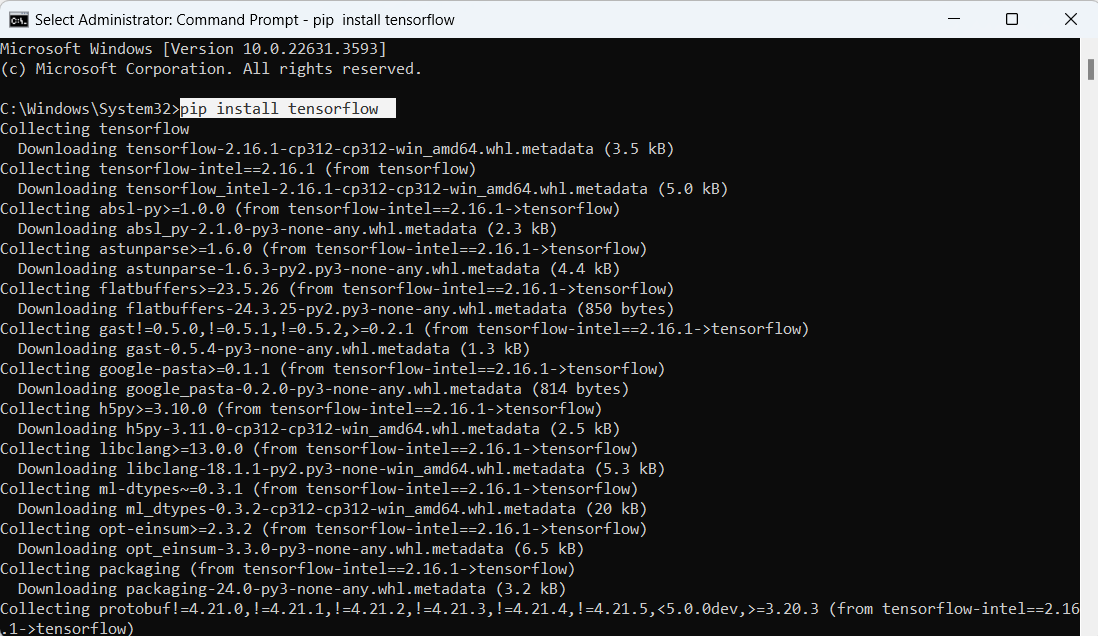
\includegraphics[width=\textwidth]{images/TensorFlowInstallation}
		\vspace{0.2cm}
		\textbf{Figure1: TensorFlow Installation}
		
		\column{0.5\textwidth}
		\centering
		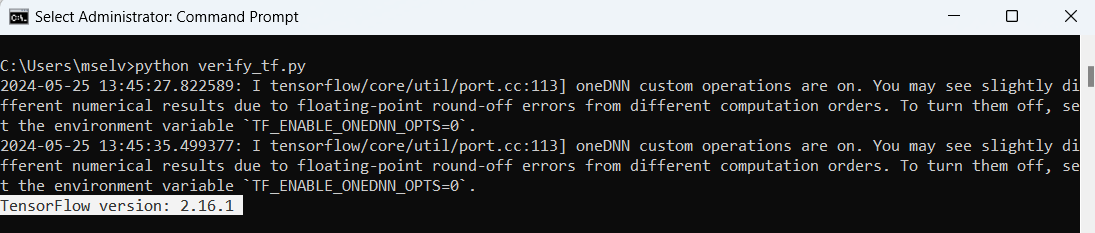
\includegraphics[width=\textwidth]{images/TensorFlowVersion}
		\vspace{0.2cm}
		\textbf{Figure2: TensorFlow Version} 
		
	\end{columns}
}

\STANDARD{Tensorflow Lite Library Installation on Arduino IDE}
{
	\begin{columns}
		\column{0.5\textwidth}
		\centering
		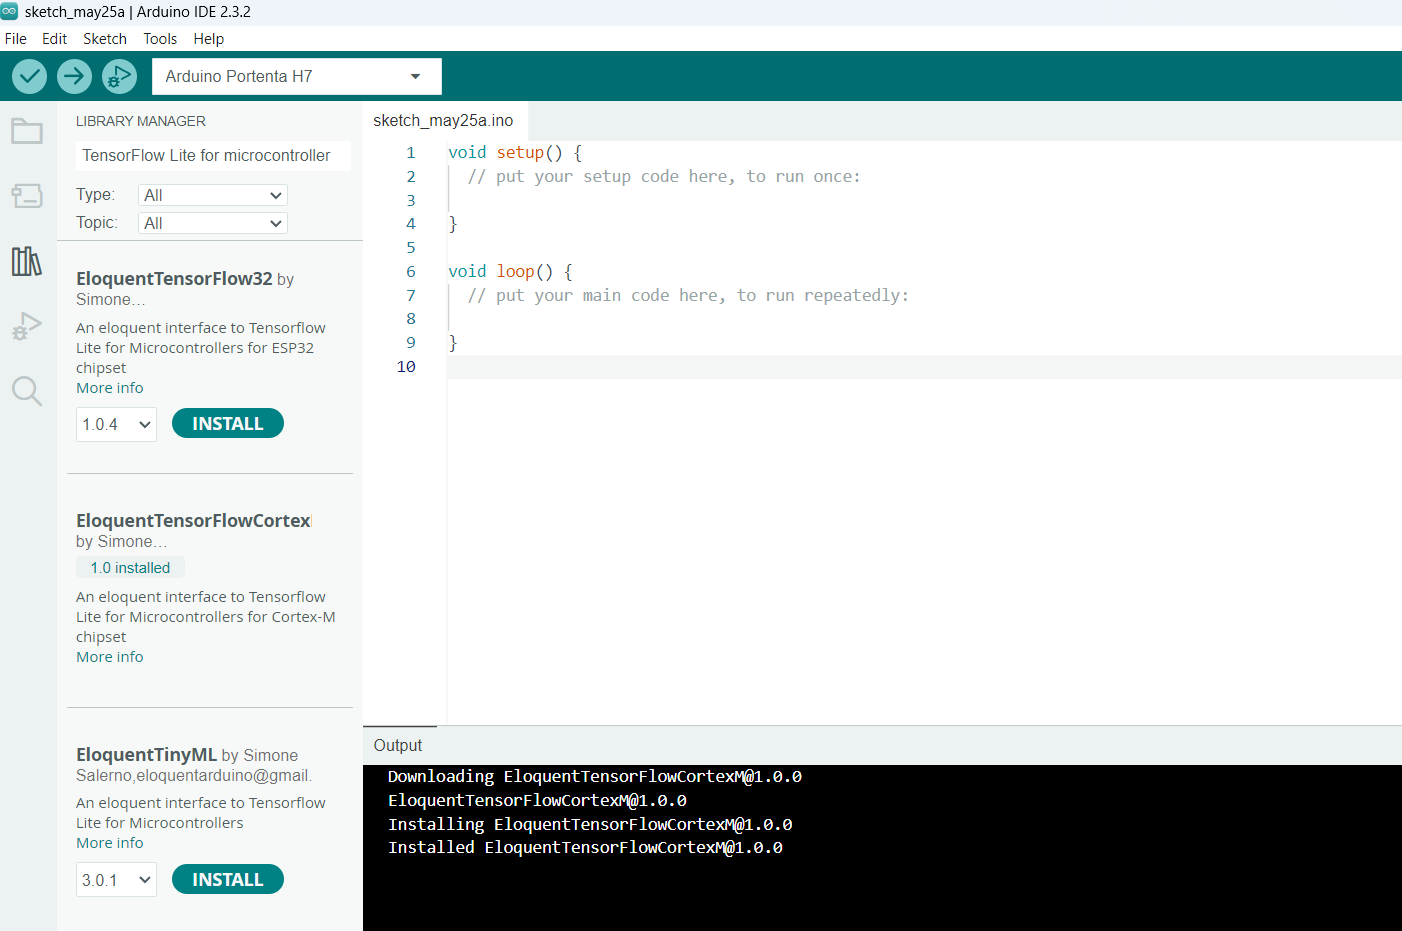
\includegraphics[width=\textwidth]{images/TensorFlowCortexLibrary}
		\vspace{0.2cm}
		\textbf{Figure1: TensorFlow Cortex Library}
		
		\column{0.5\textwidth}
		\centering
		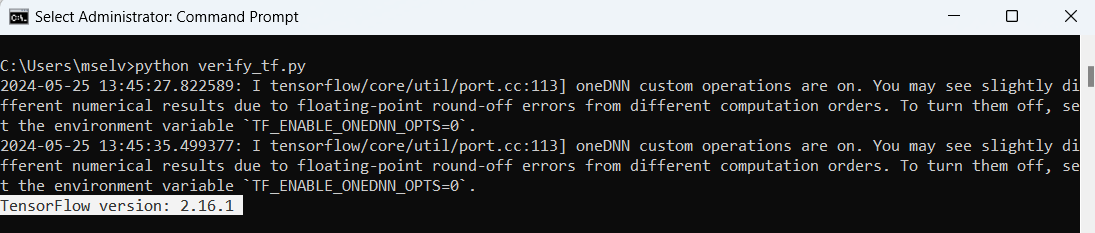
\includegraphics[width=\textwidth]{images/TensorFlowVersion}
		\vspace{0.2cm}
		\textbf{Figure2: TensorFlow Version} 
		
	\end{columns}
	
}

\begin{frame}[fragile]
	\frametitle{TensorFlow Model Training}
	
	\pythoncode{tensorflowModel.py}{Python code for training a TensorFlow model}{code:tensorflow}
	
\end{frame}

\STANDARD{STEPS}
{
	\begin{enumerate}
		\item Train a simple Keras model in TensorFlow and run the model in python to generate the file \FILE{addition\_model.h5} in the same directory of tensorflow model.
		
		\item Convert the Keras Model to TensorFlow Lite using the python script in the same directory and run the command \PYTHON{python convertModelTotflite.py} in command prompt
		
		\item Using the python script convert the TensorFlow Lite Model to a C Array and run the python \PYTHON{ConvertTfliteToHeader.py} in the command prompt
		
		\item Now include the model in the Arduino Sketch and run it on the Portenta H7.
	\end{enumerate}
}

\begin{frame}[fragile]
	\frametitle{TF Model to TF Lite}
	
	\pythoncode{convertModelTotflite.py}{Python code to convert keras model to tflite}{code:tensorflowcode}
	
\end{frame}

\begin{frame}[fragile]
	\frametitle{TF Lite Model to C Array Header}
	
	\pythoncode{ConvertTfliteToHeader.py}{Python code to convert Tensorflow Lite model to C Array}{code:tensorflowToCcode}
	
\end{frame}

\begin{frame}[fragile]{Arduino Sketch to run the model}
	
	\begin{lstlisting}[language=Python]
#include <TensorFlowLite.h>
#include <Arduino_TensorFlowLite.h>

// Include the TensorFlow Lite model
#include "simple_addition_model.h" // Assuming this is your converted model header file

void setup() {
	// Initialize serial communication
	Serial.begin(9600);
	
	// Initialize TensorFlow Lite interpreter
	if (!TfLite.begin(model_data, model_data_size)) {
		Serial.println("Failed to initialize TensorFlow Lite!");
		while (1);
	}
}
	\end{lstlisting}

\end{frame}


\begin{frame}[fragile]{Arduino Sketch to run the model}
	
	\begin{lstlisting}[language=Python]
void loop() {
	// Example inference
	float input1 = 5.0;
	float input2 = 3.0;
	
	// Prepare input tensor
	TfLiteTensor* input = TfLite.getInputTensor(0);
	input->data.f[0] = input1;
	input->data.f[1] = input2;
	
	// Run inference
	TfLite.run();
	
	// Get output tensor
	TfLiteTensor* output = TfLite.getOutputTensor(0);
	float result = output->data.f[0];
	\end{lstlisting}

\end{frame}
\begin{frame}[fragile]{Arduino Sketch to run the model}
	
	\begin{lstlisting}[language=Python]
	// Print result
	Serial.print(input1);
	Serial.print(" + ");
	Serial.print(input2);
	Serial.print(" = ");
	Serial.println(result);
	
	// Wait
	delay(1000);
}
	\end{lstlisting}
	
\end{frame}


